\chapter{Introduction}
\label{introduction}
Most audio streaming services are run by companies, incentivized to make money. They take large cuts of the subscription money from its users. As a result, the artists receive a low compensation. \todo{cite} The distributors Spotify, iTunes and Google Play take on average a 25\% cut for signed records and 40\% cut for unsigned records. This thesis investigates the feasibility and usability of an audio streaming service without a central distributor.\\

\begin{figure}
	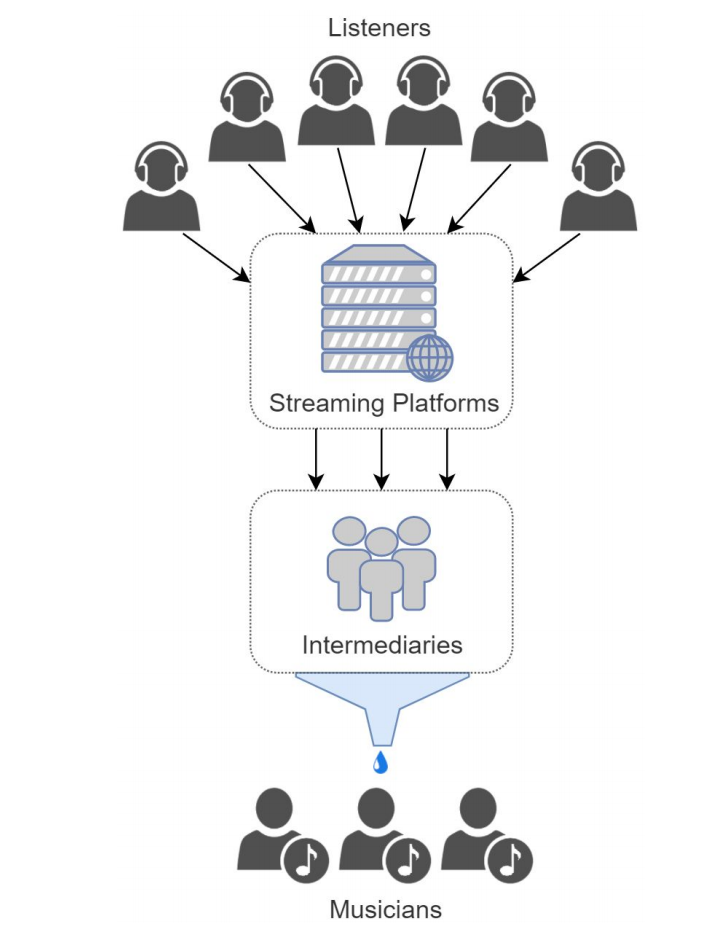
\includegraphics[width=0.4\textwidth]{./img/problem-image.png}
	\caption{Artist compensation inconsistency}
\end{figure}

This thesis proposes a solution in the form of a decentralized system which uses a decentralized autonomous organization \todo{cite}(DAO) to operate. Listeners, artists and robots form this DAO. The DAO has a shared responsibility for distributing content. In this system, its users (artists and listeners) share audio files and metadata without any middleman. Additionally, users can give donations to artists while the system does not take a cut of these donations. The user can use this system to discover, search and play audio files, targeted at music and podcasts.\\

\todo{XYZ} Section X describes the design of the system, section Y its implementation and Z its testing results.